\begin{frame}
  \begin{center}
    {\bf Hands-on: Exploiting Weaknesses in RSA}\\
    {\bf -- at bigger scale --}\\
  \end{center}
\end{frame}

\begin{frame}
  \frametitle{Snake Oil Crypto\footnote{\url{https://github.com/d4-project/snake-oil-crypto}} - Problem Statement}
  We reckon that IoT devices {\bf are often the weakest devices} on a network:

        \begin{itemize}
        \item Usually the result of cheap engineering,
        \item sloppy patching cycles,
        \item sometimes forgotten--not monitored (remember the printer sending sysmon?),
        \item few hardening features enabled.
        \end{itemize}

        \vspace{10 mm} 

{\bf We feel a bit safer when they use TLS, but we what you now know about RSA, should we?}
\end{frame}

\begin{frame}
   \frametitle{Snake Oil Crypto - GCD}
   In Snake-Oil-Crypto we compute GCD\footnote{using Bernstein's Batch GCD algorithm} between:
   
   \begin{itemize}
     \item between certificates having the same issuer,
     \item between certificates having the same subject,
     \item on keys collected from various sources (PassiveSSL, Certificate Transparency,
       shodan, censys, etc.),
     \item python + redis + postgresql~\footnote{\url{https://github.com/D4-project/snake-oil-crypto/}}
   \end{itemize}

\vspace{10 mm}
  {\bf ``Check all the keys that we know of for vendor X''}

\end{frame}

\begin{frame}
   \frametitle{Snake Oil Crypto - GCD}

   Quick Demo:
   \begin{itemize}
   \item Let's check how strong are the RSA keys in our database...
   \item check some results on https://misp-eurolea.enforce.lan
   \item how bad can it be?
   \item do you find some vendors we should notify?
   \end{itemize}

\end{frame}

\begin{frame}
   \frametitle{Snake Oil Crypto - MISP feed}
\begin{figure}
\centering
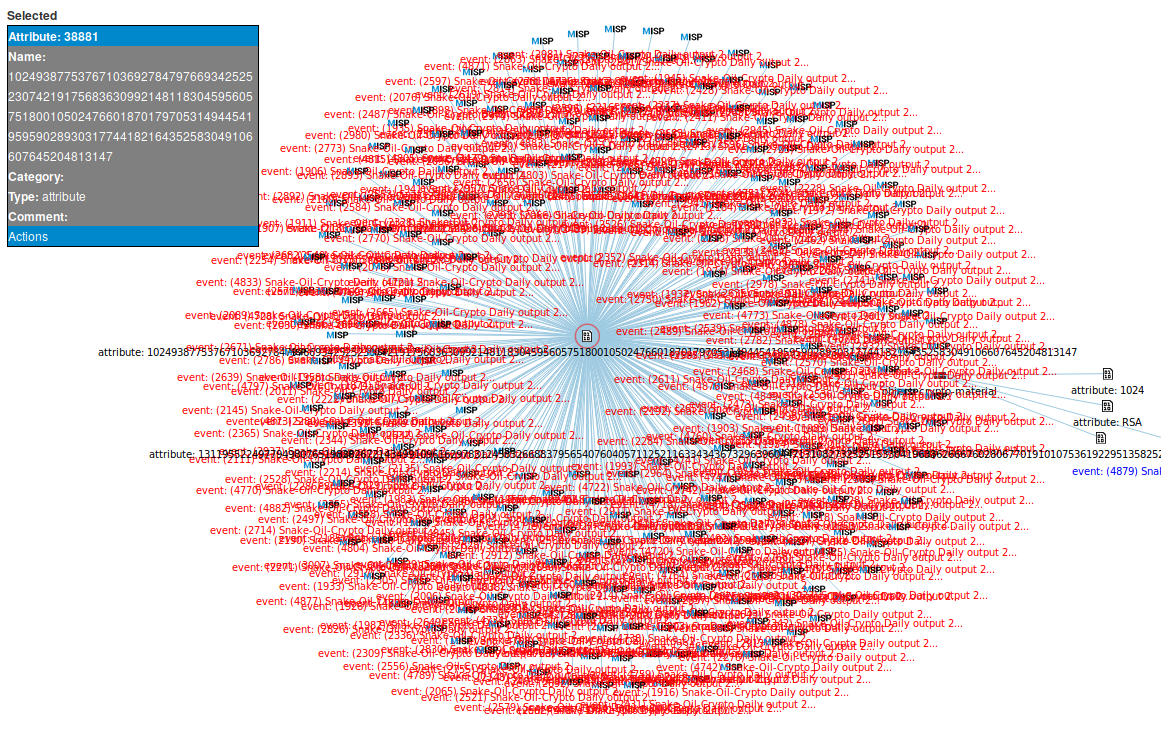
\includegraphics[width=\textwidth]{misp.png}
\end{figure}
\end{frame}

\begin{frame}
   \frametitle{Snake Oil Crypto - MISP feed}
   The MISP feed:
   \begin{itemize}
     \item {\bf Allows} for checking automatic checking by an IDS on hashed values,
     \item {\bf contains} thousands on broken keys from a dozen of vendors,
     \item {\bf will be accessible upon request (info@circl.lu).}
   \end{itemize}

   In the future:
    \begin{itemize}
     \item {\bf Automatic} the vendor checks by performing TF-IDF on x509's subjects, 
     \item {\bf automatic} vendors notification.
    \end{itemize}

\end{frame}
